% Options for packages loaded elsewhere
\PassOptionsToPackage{unicode}{hyperref}
\PassOptionsToPackage{hyphens}{url}
%
\documentclass[
]{article}
\usepackage{lmodern}
\usepackage{amssymb,amsmath}
\usepackage{ifxetex,ifluatex}
\ifnum 0\ifxetex 1\fi\ifluatex 1\fi=0 % if pdftex
  \usepackage[T1]{fontenc}
  \usepackage[utf8]{inputenc}
  \usepackage{textcomp} % provide euro and other symbols
\else % if luatex or xetex
  \usepackage{unicode-math}
  \defaultfontfeatures{Scale=MatchLowercase}
  \defaultfontfeatures[\rmfamily]{Ligatures=TeX,Scale=1}
\fi
% Use upquote if available, for straight quotes in verbatim environments
\IfFileExists{upquote.sty}{\usepackage{upquote}}{}
\IfFileExists{microtype.sty}{% use microtype if available
  \usepackage[]{microtype}
  \UseMicrotypeSet[protrusion]{basicmath} % disable protrusion for tt fonts
}{}
\makeatletter
\@ifundefined{KOMAClassName}{% if non-KOMA class
  \IfFileExists{parskip.sty}{%
    \usepackage{parskip}
  }{% else
    \setlength{\parindent}{0pt}
    \setlength{\parskip}{6pt plus 2pt minus 1pt}}
}{% if KOMA class
  \KOMAoptions{parskip=half}}
\makeatother
\usepackage{xcolor}
\IfFileExists{xurl.sty}{\usepackage{xurl}}{} % add URL line breaks if available
\IfFileExists{bookmark.sty}{\usepackage{bookmark}}{\usepackage{hyperref}}
\hypersetup{
  pdftitle={기호 수학(Symbolic Math)},
  hidelinks,
  pdfcreator={LaTeX via pandoc}}
\urlstyle{same} % disable monospaced font for URLs
\usepackage[margin=1in]{geometry}
\usepackage{color}
\usepackage{fancyvrb}
\newcommand{\VerbBar}{|}
\newcommand{\VERB}{\Verb[commandchars=\\\{\}]}
\DefineVerbatimEnvironment{Highlighting}{Verbatim}{commandchars=\\\{\}}
% Add ',fontsize=\small' for more characters per line
\usepackage{framed}
\definecolor{shadecolor}{RGB}{248,248,248}
\newenvironment{Shaded}{\begin{snugshade}}{\end{snugshade}}
\newcommand{\AlertTok}[1]{\textcolor[rgb]{0.94,0.16,0.16}{#1}}
\newcommand{\AnnotationTok}[1]{\textcolor[rgb]{0.56,0.35,0.01}{\textbf{\textit{#1}}}}
\newcommand{\AttributeTok}[1]{\textcolor[rgb]{0.77,0.63,0.00}{#1}}
\newcommand{\BaseNTok}[1]{\textcolor[rgb]{0.00,0.00,0.81}{#1}}
\newcommand{\BuiltInTok}[1]{#1}
\newcommand{\CharTok}[1]{\textcolor[rgb]{0.31,0.60,0.02}{#1}}
\newcommand{\CommentTok}[1]{\textcolor[rgb]{0.56,0.35,0.01}{\textit{#1}}}
\newcommand{\CommentVarTok}[1]{\textcolor[rgb]{0.56,0.35,0.01}{\textbf{\textit{#1}}}}
\newcommand{\ConstantTok}[1]{\textcolor[rgb]{0.00,0.00,0.00}{#1}}
\newcommand{\ControlFlowTok}[1]{\textcolor[rgb]{0.13,0.29,0.53}{\textbf{#1}}}
\newcommand{\DataTypeTok}[1]{\textcolor[rgb]{0.13,0.29,0.53}{#1}}
\newcommand{\DecValTok}[1]{\textcolor[rgb]{0.00,0.00,0.81}{#1}}
\newcommand{\DocumentationTok}[1]{\textcolor[rgb]{0.56,0.35,0.01}{\textbf{\textit{#1}}}}
\newcommand{\ErrorTok}[1]{\textcolor[rgb]{0.64,0.00,0.00}{\textbf{#1}}}
\newcommand{\ExtensionTok}[1]{#1}
\newcommand{\FloatTok}[1]{\textcolor[rgb]{0.00,0.00,0.81}{#1}}
\newcommand{\FunctionTok}[1]{\textcolor[rgb]{0.00,0.00,0.00}{#1}}
\newcommand{\ImportTok}[1]{#1}
\newcommand{\InformationTok}[1]{\textcolor[rgb]{0.56,0.35,0.01}{\textbf{\textit{#1}}}}
\newcommand{\KeywordTok}[1]{\textcolor[rgb]{0.13,0.29,0.53}{\textbf{#1}}}
\newcommand{\NormalTok}[1]{#1}
\newcommand{\OperatorTok}[1]{\textcolor[rgb]{0.81,0.36,0.00}{\textbf{#1}}}
\newcommand{\OtherTok}[1]{\textcolor[rgb]{0.56,0.35,0.01}{#1}}
\newcommand{\PreprocessorTok}[1]{\textcolor[rgb]{0.56,0.35,0.01}{\textit{#1}}}
\newcommand{\RegionMarkerTok}[1]{#1}
\newcommand{\SpecialCharTok}[1]{\textcolor[rgb]{0.00,0.00,0.00}{#1}}
\newcommand{\SpecialStringTok}[1]{\textcolor[rgb]{0.31,0.60,0.02}{#1}}
\newcommand{\StringTok}[1]{\textcolor[rgb]{0.31,0.60,0.02}{#1}}
\newcommand{\VariableTok}[1]{\textcolor[rgb]{0.00,0.00,0.00}{#1}}
\newcommand{\VerbatimStringTok}[1]{\textcolor[rgb]{0.31,0.60,0.02}{#1}}
\newcommand{\WarningTok}[1]{\textcolor[rgb]{0.56,0.35,0.01}{\textbf{\textit{#1}}}}
\usepackage{longtable,booktabs}
% Correct order of tables after \paragraph or \subparagraph
\usepackage{etoolbox}
\makeatletter
\patchcmd\longtable{\par}{\if@noskipsec\mbox{}\fi\par}{}{}
\makeatother
% Allow footnotes in longtable head/foot
\IfFileExists{footnotehyper.sty}{\usepackage{footnotehyper}}{\usepackage{footnote}}
\makesavenoteenv{longtable}
\usepackage{graphicx}
\makeatletter
\def\maxwidth{\ifdim\Gin@nat@width>\linewidth\linewidth\else\Gin@nat@width\fi}
\def\maxheight{\ifdim\Gin@nat@height>\textheight\textheight\else\Gin@nat@height\fi}
\makeatother
% Scale images if necessary, so that they will not overflow the page
% margins by default, and it is still possible to overwrite the defaults
% using explicit options in \includegraphics[width, height, ...]{}
\setkeys{Gin}{width=\maxwidth,height=\maxheight,keepaspectratio}
% Set default figure placement to htbp
\makeatletter
\def\fps@figure{htbp}
\makeatother
\setlength{\emergencystretch}{3em} % prevent overfull lines
\providecommand{\tightlist}{%
  \setlength{\itemsep}{0pt}\setlength{\parskip}{0pt}}
\setcounter{secnumdepth}{-\maxdimen} % remove section numbering
\usepackage{tikz}
\usepackage{pgfplots}
\ifluatex
  \usepackage{selnolig}  % disable illegal ligatures
\fi

\title{기호 수학(Symbolic Math)}
\usepackage{etoolbox}
\makeatletter
\providecommand{\subtitle}[1]{% add subtitle to \maketitle
  \apptocmd{\@title}{\par {\large #1 \par}}{}{}
}
\makeatother
\subtitle{R마크다운 - 기하 저작}
\author{true}
\date{2021-02-13}

\begin{document}
\maketitle

\hypertarget{geometry-symbols}{%
\section{기하 기호}\label{geometry-symbols}}

기하학에서 자주 사용되는 수학기소는 다음과 같다.

\begin{longtable}[]{@{}ccc@{}}
\toprule
의미 & 수학기호 & \(\LaTeX\)\tabularnewline
\midrule
\endhead
선분(Line Segment) & \(\overline{\rm AB}\) &
\textbackslash overline\{\textbackslash rm AB\}\tabularnewline
각(Angle) & \(\angle\) & \textbackslash angle\tabularnewline
측정된 각(Measured Angle) & \(\measuredangle\) &
\textbackslash measuredangle\tabularnewline
삼각형(Triangle) & \(\triangle\) &
\textbackslash triangle\tabularnewline
정사각형(Square) & \(\square\) & \textbackslash square\tabularnewline
합동( congruent ): 같은 모양, 크기 & \(\cong\) &
\textbackslash cong\tabularnewline
닮음(similar, same shape) & \(\sim\) & \textbackslash sim\tabularnewline
평행(is parallel with) & \(\|\) &
\textbackslash\textbar{}\tabularnewline
수선(perpendicular): 어떤 일정한 직선 또는 평면에 수직인 직선 &
\(\perp\) & \textbackslash perp\tabularnewline
\bottomrule
\end{longtable}

\hypertarget{math-geometry}{%
\section[다양한 수학 도형]{\texorpdfstring{다양한 수학
도형\footnote{\href{https://stackoverflow.com/questions/51689570/how-to-force-tikz-in-rmarkdown-document-to-show-cyrillic-text}{``How
  to force Tikz in RMarkdown document to show cyrillic text?'',
  stackoverflow}}}{다양한 수학 도형}}\label{math-geometry}}

\begin{Shaded}
\begin{Highlighting}[]

\KeywordTok{\textbackslash{}begin}\NormalTok{\{}\ExtensionTok{tikzpicture}\NormalTok{\}}
\KeywordTok{\textbackslash{}begin}\NormalTok{\{}\ExtensionTok{scope}\NormalTok{\}[blend group = soft light]}
  \FunctionTok{\textbackslash{}fill}\NormalTok{[red!30!white]   ( 90:1.2) circle (2);}
  \FunctionTok{\textbackslash{}fill}\NormalTok{[green!30!white] (210:1.2) circle (2);}
  \FunctionTok{\textbackslash{}fill}\NormalTok{[blue!30!white]  (330:1.2) circle (2);}
\KeywordTok{\textbackslash{}end}\NormalTok{\{}\ExtensionTok{scope}\NormalTok{\}}
\FunctionTok{\textbackslash{}node}\NormalTok{ at ( 90:2)    \{Statistics\};}
\FunctionTok{\textbackslash{}node}\NormalTok{ at ( 210:2)   \{Mathematics\};}
\FunctionTok{\textbackslash{}node}\NormalTok{ at ( 330:2)   \{Coding\};}
\FunctionTok{\textbackslash{}node}\NormalTok{ [font=}\FunctionTok{\textbackslash{}Large}\NormalTok{] \{Data Science\};}
\KeywordTok{\textbackslash{}end}\NormalTok{\{}\ExtensionTok{tikzpicture}\NormalTok{\}}
\end{Highlighting}
\end{Shaded}

\begin{center}\includegraphics{math-history-geometry-md_files/figure-latex/make-data-science-1} \end{center}

\hypertarget{triangle}{%
\subsection{직각 삼각형}\label{triangle}}

\texttt{tikz} \(\LaTeX\) 팩키지를 사용해서 직각삼각형을 그려보자.

\begin{Shaded}
\begin{Highlighting}[]
\KeywordTok{\textbackslash{}begin}\NormalTok{\{}\ExtensionTok{tikzpicture}\NormalTok{\}[scale=1.25]}

    \FunctionTok{\textbackslash{}coordinate}\NormalTok{ [label = left:}\SpecialStringTok{$C$}\NormalTok{]  (A) at (0,0);}
    \FunctionTok{\textbackslash{}coordinate}\NormalTok{ [label = right:}\SpecialStringTok{$A$}\NormalTok{] (C) at (3,0);}
    \FunctionTok{\textbackslash{}coordinate}\NormalTok{ [label = above:}\SpecialStringTok{$B$}\NormalTok{] (B) at (3,3);}
    
    \FunctionTok{\textbackslash{}draw}\NormalTok{             (A) {-}{-}}
\NormalTok{    node[above] \{}\SpecialStringTok{$a$}\NormalTok{\} (B) {-}{-}}
\NormalTok{    node[right] \{}\SpecialStringTok{$c$}\NormalTok{\} (C) {-}{-} }
\NormalTok{    node[below] \{}\SpecialStringTok{$b$}\NormalTok{\} (A);}
    
    \FunctionTok{\textbackslash{}draw}\NormalTok{ (3, 0) rectangle (2.7, 0.3);}

\KeywordTok{\textbackslash{}end}\NormalTok{\{}\ExtensionTok{tikzpicture}\NormalTok{\}}
\end{Highlighting}
\end{Shaded}

\begin{center}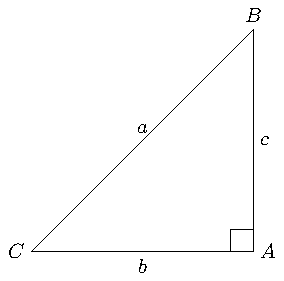
\includegraphics{math-history-geometry-md_files/figure-latex/draw-triangle-1} \end{center}

상기 \texttt{tikz} \(\LaTeX\) 코드 대신 삼각형을 \texttt{ggplot}으로
그려보자. \texttt{geom\_segment()}, \texttt{geom\_point()}를 사용하여
기하도형을 그리고 \texttt{annotate()}로 삼각형의 기호를 표시한다.

\begin{Shaded}
\begin{Highlighting}[]
\KeywordTok{library}\NormalTok{(tidyverse)}

\KeywordTok{ggplot}\NormalTok{() }\OperatorTok{+}
\StringTok{  }\CommentTok{\# 선분 AB, BC, CA}
\StringTok{  }\KeywordTok{geom\_segment}\NormalTok{(}\KeywordTok{aes}\NormalTok{(}\DataTypeTok{x=}\DecValTok{0}\NormalTok{, }\DataTypeTok{y =} \DecValTok{0}\NormalTok{, }\DataTypeTok{xend =} \DecValTok{3}\NormalTok{, }\DataTypeTok{yend =} \DecValTok{0}\NormalTok{)) }\OperatorTok{+}
\StringTok{  }\KeywordTok{geom\_segment}\NormalTok{(}\KeywordTok{aes}\NormalTok{(}\DataTypeTok{x=}\DecValTok{3}\NormalTok{, }\DataTypeTok{y =} \DecValTok{0}\NormalTok{, }\DataTypeTok{xend =} \DecValTok{3}\NormalTok{, }\DataTypeTok{yend =} \DecValTok{3}\NormalTok{)) }\OperatorTok{+}
\StringTok{  }\KeywordTok{geom\_segment}\NormalTok{(}\KeywordTok{aes}\NormalTok{(}\DataTypeTok{x=}\DecValTok{3}\NormalTok{, }\DataTypeTok{y =} \DecValTok{3}\NormalTok{, }\DataTypeTok{xend =} \DecValTok{0}\NormalTok{, }\DataTypeTok{yend =} \DecValTok{0}\NormalTok{)) }\OperatorTok{+}
\StringTok{  }\CommentTok{\# 점 A, B, C}
\StringTok{  }\KeywordTok{geom\_point}\NormalTok{(}\KeywordTok{aes}\NormalTok{(}\DataTypeTok{x=}\DecValTok{0}\NormalTok{, }\DataTypeTok{y=}\DecValTok{0}\NormalTok{), }\DataTypeTok{size =} \DecValTok{3}\NormalTok{) }\OperatorTok{+}
\StringTok{  }\KeywordTok{geom\_point}\NormalTok{(}\KeywordTok{aes}\NormalTok{(}\DataTypeTok{x=}\DecValTok{3}\NormalTok{, }\DataTypeTok{y=}\DecValTok{0}\NormalTok{), }\DataTypeTok{size =} \DecValTok{3}\NormalTok{) }\OperatorTok{+}
\StringTok{  }\KeywordTok{geom\_point}\NormalTok{(}\KeywordTok{aes}\NormalTok{(}\DataTypeTok{x=}\DecValTok{3}\NormalTok{, }\DataTypeTok{y=}\DecValTok{3}\NormalTok{), }\DataTypeTok{size =} \DecValTok{3}\NormalTok{) }\OperatorTok{+}
\StringTok{  }\CommentTok{\# 점에 라벨 붙이기}
\StringTok{  }\KeywordTok{annotate}\NormalTok{(}\StringTok{"text"}\NormalTok{, }\DataTypeTok{x =} \DecValTok{0}\NormalTok{, }\DataTypeTok{y=} \DecValTok{0}\NormalTok{, }\DataTypeTok{label =} \StringTok{"C"}\NormalTok{, }\DataTypeTok{hjust =}  \DecValTok{2}\NormalTok{, }\DataTypeTok{size =} \DecValTok{5}\NormalTok{) }\OperatorTok{+}
\StringTok{  }\KeywordTok{annotate}\NormalTok{(}\StringTok{"text"}\NormalTok{, }\DataTypeTok{x =} \DecValTok{3}\NormalTok{, }\DataTypeTok{y=} \DecValTok{0}\NormalTok{, }\DataTypeTok{label =} \StringTok{"A"}\NormalTok{, }\DataTypeTok{hjust =} \DecValTok{{-}1}\NormalTok{, }\DataTypeTok{size =} \DecValTok{5}\NormalTok{) }\OperatorTok{+}
\StringTok{  }\KeywordTok{annotate}\NormalTok{(}\StringTok{"text"}\NormalTok{, }\DataTypeTok{x =} \DecValTok{3}\NormalTok{, }\DataTypeTok{y=} \DecValTok{3}\NormalTok{, }\DataTypeTok{label =} \StringTok{"B"}\NormalTok{, }\DataTypeTok{vjust =} \DecValTok{{-}1}\NormalTok{, }\DataTypeTok{size =} \DecValTok{5}\NormalTok{) }\OperatorTok{+}
\StringTok{  }\CommentTok{\# 선분에 라벨 붙이기}
\StringTok{  }\KeywordTok{annotate}\NormalTok{(}\StringTok{"text"}\NormalTok{, }\DataTypeTok{x =} \FloatTok{1.5}\NormalTok{, }\DataTypeTok{y =} \FloatTok{0.0}\NormalTok{, }\DataTypeTok{label =} \StringTok{"italic(b)"}\NormalTok{, }\DataTypeTok{vjust =}  \DecValTok{1}\NormalTok{, }\DataTypeTok{size =} \DecValTok{5}\NormalTok{, }\DataTypeTok{parse =} \OtherTok{TRUE}\NormalTok{) }\OperatorTok{+}
\StringTok{  }\KeywordTok{annotate}\NormalTok{(}\StringTok{"text"}\NormalTok{, }\DataTypeTok{x =} \FloatTok{3.0}\NormalTok{, }\DataTypeTok{y =} \FloatTok{1.5}\NormalTok{, }\DataTypeTok{label =} \StringTok{"italic(c)"}\NormalTok{, }\DataTypeTok{hjust =} \DecValTok{{-}1}\NormalTok{, }\DataTypeTok{size =} \DecValTok{5}\NormalTok{, }\DataTypeTok{parse =} \OtherTok{TRUE}\NormalTok{) }\OperatorTok{+}
\StringTok{  }\KeywordTok{annotate}\NormalTok{(}\StringTok{"text"}\NormalTok{, }\DataTypeTok{x =} \FloatTok{1.5}\NormalTok{, }\DataTypeTok{y =} \FloatTok{1.5}\NormalTok{, }\DataTypeTok{label =} \StringTok{"italic(a)"}\NormalTok{, }\DataTypeTok{vjust =} \DecValTok{{-}1}\NormalTok{, }\DataTypeTok{size =} \DecValTok{5}\NormalTok{, }\DataTypeTok{parse =} \OtherTok{TRUE}\NormalTok{) }\OperatorTok{+}
\StringTok{  }\CommentTok{\# 직각 표시}
\StringTok{  }\KeywordTok{geom\_segment}\NormalTok{(}\KeywordTok{aes}\NormalTok{(}\DataTypeTok{x=}\FloatTok{2.9}\NormalTok{, }\DataTypeTok{y =} \FloatTok{0.0}\NormalTok{, }\DataTypeTok{xend =} \FloatTok{2.9}\NormalTok{, }\DataTypeTok{yend =} \FloatTok{0.1}\NormalTok{)) }\OperatorTok{+}
\StringTok{  }\KeywordTok{geom\_segment}\NormalTok{(}\KeywordTok{aes}\NormalTok{(}\DataTypeTok{x=}\FloatTok{2.9}\NormalTok{, }\DataTypeTok{y =} \FloatTok{0.1}\NormalTok{, }\DataTypeTok{xend =} \FloatTok{3.0}\NormalTok{, }\DataTypeTok{yend =} \FloatTok{0.1}\NormalTok{)) }\OperatorTok{+}
\StringTok{  }\KeywordTok{theme\_void}\NormalTok{() }\OperatorTok{+}
\StringTok{  }\KeywordTok{coord\_equal}\NormalTok{(}\DataTypeTok{ratio =} \DecValTok{1}\NormalTok{) }\OperatorTok{+}
\StringTok{  }\KeywordTok{scale\_x\_continuous}\NormalTok{(}\DataTypeTok{limits =} \KeywordTok{c}\NormalTok{(}\OperatorTok{{-}}\FloatTok{0.5}\NormalTok{, }\FloatTok{3.5}\NormalTok{)) }\OperatorTok{+}
\StringTok{  }\KeywordTok{scale\_y\_continuous}\NormalTok{(}\DataTypeTok{limits =} \KeywordTok{c}\NormalTok{(}\OperatorTok{{-}}\FloatTok{0.5}\NormalTok{, }\FloatTok{3.5}\NormalTok{))}
\end{Highlighting}
\end{Shaded}

\begin{center}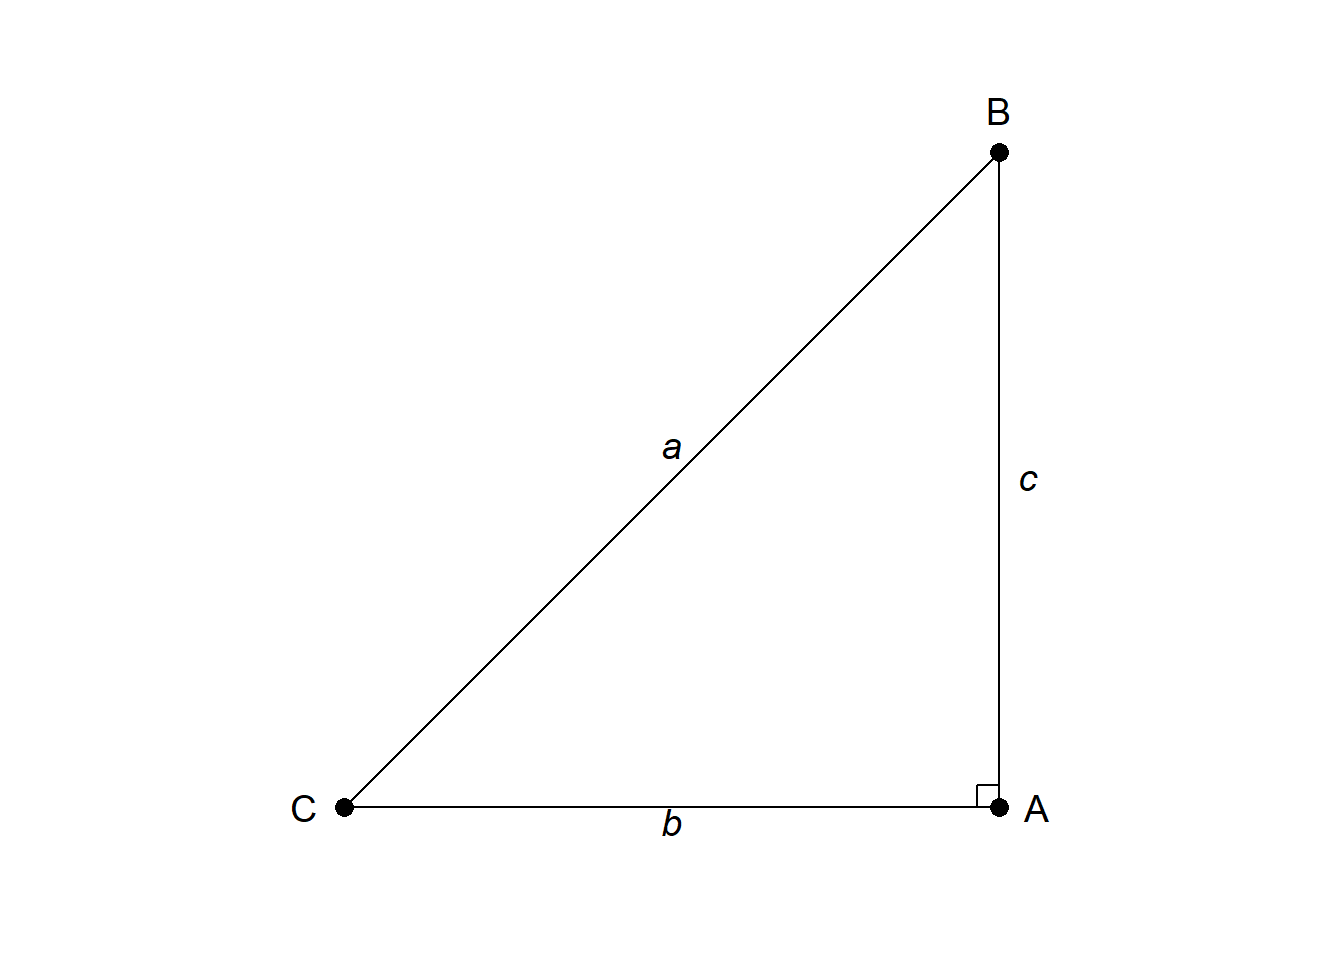
\includegraphics{math-history-geometry-md_files/figure-latex/draw-ggplot-1} \end{center}

\end{document}
